\section{序論}\label{ux5e8fux8ad6}

これはテンプレートです。\texttt{src/thesis.md}
を編集してプッシュすると、自動でPDFが更新されます。

\subsection{数式の例}\label{ux6570ux5f0fux306eux4f8b}

式\eqref{eq:sample}は重要な式です。

\begin{equation}
  e^{i\pi} + 1 = 0 \label{eq:sample}
\end{equation}

\subsection{図の例}\label{ux56f3ux306eux4f8b}

図\ref{fig:dummy}を参照してください。画像は \texttt{src/images}
に入れてください。

\begin{figure}
\centering
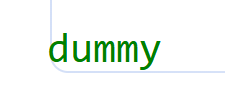
\includegraphics{images/dummy.png}
\caption{ダミー画像 \label{fig:dummy}}
\end{figure}

\subsection{参考文献の例}\label{ux53c2ux8003ux6587ux732eux306eux4f8b}

GitHub Actionsは便利である \citep{doe2025}。
